\chapter{Technical summary}

This chapter summarizes the technical details associated with producing this report. It shows various schemas and dependencies that explain the overall structure of the whole data pipeline. Two programming languages were used for the process - R and Python. The R code is responsible for downloading the raw data, cleaning it and exporting the relevant parts. The Python code is responsible for converting the data into a lightweight format, creating and exporting the figures and compiling the final version of the report. All in all, one could say that the R part handles the data while the Python part handles the plotting and latex compilation. A visual representation of the process can be found in Figure \ref{fig:technical_summary:flowcharts_R_python}. Further details regarding specific functions and their roles can be found in tables \ref{tab:technical_summary:used_functions_R} and \ref{tab:technical_summary:used_functions_python}.

\begin{table}[h]
	\centering
	\begin{tabularx}{0.9\linewidth}{rX}
		Function name & Description \\
		\toprule
		\textbf{download\_MMSR\_data.R} & Downloads the MMSR dataset, stores it in its raw form as a large number of xml files. \\
		\textbf{redownload\_MMSR\_data.R} & A failsafe that tries to download xml files that the main download function might have missed due to connection or server issues \\
		\textbf{parse\_MMSR\_data.R} & Translates every downloaded xml file into an RData file to allow further data wrangling.  \\
		\textbf{combine\_MMSR\_data.R} & Combines the translated .RData files into monthly and yearly datasets which are in turn combined into two full datasets - one for the secured and one for the unsecured segment. Only keeps variables that are relevant for the analysis.   \\
		\textbf{prepare\_MMSR\_data.R} & Imports a full MMSR segment, removes erroneous observations, merges fixed and variable rates into a single variable, calculates maturity in business and calendar days, only keeps observations that are within the time period that we are interested in, saves the resulting dataset in multiple granularities (granular, daily, weekly, monthly) and multiple formats (.RData, .csv).\\
		\textbf{prepare\_network\_data.R} & Brackets observations by reporting agents, creates individual categories for CCPs, computes network of monthly volume exposures across pairs of agents. Creates a dataset depicting the evolution of different network centrality measures for each agent. (.RData, .csv).\\
		\textbf{functions.R} & Contains the dedicated xml parser used to translate a single xml page into an R dataframe of the correct format. \\
		\bottomrule
	\end{tabularx}
	\caption{R functions used in the analysis.}
	\label{tab:technical_summary:used_functions_R}
\end{table}

\section{Data handling}
The MMSR data is located on a dedicated server which is accessible by user's DARWIN credentials after a proper registration / data request. From this server, the data can be downloaded by directly saving an xml file with the relevant transaction details. The whole process of the data transformation within my pipeline can be seen on the left hand side of Figure \ref{fig:technical_summary:flowcharts_R_python}. I will describe the relevant steps in further detail now.

\subsection{Download}
The first step is the data download. For this purpose, we use the function \verb|download_MMSR_data.R|. This function fulfills the following tasks:
\begin{enumerate}
	\item Specifies the segment to be downloaded (secured or unsecured).
	\item Asks the user for their DARWIN credentials and stores them in a non-human-readable binary format.
	\item Creates the directory structure for the downloaded data. 
	\item Downloads the relevant xml files. Each xml file corresponds to 100 transactions on a given day, therefore the data for one day of MMSR data will likely consist of tens / hundreds of xml files. These files are saved in the created directory structure where each file's location is \ \ \verb|data/[segment]/data_raw/[year]/[month]/[day]/[page number].xml|.
	\item For each trading day, the function creates a text file that stores the total number of xml files for this particular day. The file is stored as \newline \verb|data/[segment]/data_raw/[year]/[month]/[day]/number_of_pages.txt|.
\end{enumerate}

\subsection{Download check}
In the second step, we use the function \verb|redownload_MMSR_data.R| which goes through the downloaded files and attempts to download missing data. It's possible that due to connection or server issues, some xml files have not been downloaded in the previous step. The way this function solves this issue is as follows:
\begin{enumerate}
	\item For each trading day, the function reads the file \verb|number_of_pages.txt| to determine the number of available xml files for that day $X$. If there were connection issues at this moment in the data download before, there could be further xml files for this day. Therefore, the function then attempts to download the xml file number $X+1$. If it succeeds, it continues to download further xml files at $X+2, X+3, \ldots$ until the relevant page no longer exists. In that case, it changes the value of $X$ in \verb|number_of_pages.txt| and then moves on to the next day.
	\item After checking all days in the relevant period, the function prints the number of new xml files that have been downloaded. If this number is greater than zero, it means some pages have been added which we did not have previously due to connection / server issues. It would be a good practice to run this function several times in the span of a few days to make sure there is no more data at the server. Unfortunately there is not a better way to know.
\end{enumerate}


\begin{table}[h]
	\centering
	\begin{tabularx}{0.9\linewidth}{rXc}
		\toprule
		\textbf{year} & Year of the transaction settlement  &numeric \\
		\textbf{quarter} & Quarter of the transaction settlement  &numeric\\
		\textbf{month} & Month of the transaction settlement  &numeric\\
		\textbf{week} & Week of the transaction settlement  &numeric\\
		\textbf{settlement\_date} & Day of the transaction settlement  &date\\		
		\textbf{report\_agent\_lei} & Reporting bank's unique identifier  &character\\
		\textbf{report\_agent\_loc} & Reporting bank's location code  &character\\
		\textbf{report\_agent\_name} & Reporting bank's name  &character\\
		\textbf{cntp\_sector} & Reporting bank's unique identifier  &character\\
		\textbf{cntp\_lei} & Unique identifier of the transaction counter-party  &character\\
		\textbf{cntp\_loc\_code} & Location of the transaction counter-party  &character\\
		\textbf{trns\_type} & Type of the transaction, BORR or LEND.  &character\\
		\textbf{maturity\_date} & Maturity day of the transaction  &date\\
		\textbf{trns\_nominal\_amt} & Transaction amount  &numeric\\
		\textbf{cntp\_ccp\_flag} & Binary variable that determines whether the counterparty is a central clearing party - CCP  &binary\\
		\textbf{rate} & Interest rate on the transaction p.a.  &numeric\\
		\textbf{maturity} & Number of business days until between the settlement date and the maturity date  &numeric\\
		\textbf{maturity\_calendar} & Number of calendar days until between the settlement date and the maturity date  &numeric\\
		\bottomrule
	\end{tabularx}
	\caption{Variables used in the analysis.}
	\label{tab:technical_summary:used_variables}
\end{table}

\subsection{Parsing}
In the third step, we use the function \verb|parse_MMSR_data.R|. This function leverages our parsing script from \verb|functions.R| to translate the xml files into R dataframes.
\begin{enumerate}
	\item Specifies the segment to be parsed (secured or unsecured).
	\item Specifies the sample data file to understand the data structure. This is a preemptive measure against future changes in MMSR data structure (new variables added, old variables removed etc.)
	\item Reads the xml files saved in the previous step, imports them into R, merges xml pages from the same day into a single dataframe and saves these dataframes into a new folder structure. In this new directory structure, each file is located at \newline \verb|data/[segment]/data_parsed/[year]/[month]/[day].RData|.
\end{enumerate}

\subsection{Merging}
In the fourth step, we use the function \verb|combine_MMSR_data.R|. This function combines the dataframes into chunks of monthly and yearly datasets, also creating one single dataframe for each segment.
\begin{enumerate}
	\item Specifies the segment to be merged (secured or unsecured).
	\item Specifies the variables relevant for the analysis and this report and drops the rest. Variables that are being kept can be found in Table \ref{tab:technical_summary:used_variables}.
	\item Goes through all saved dataframes and creates a new directory structure with merged data. In this new directory structure, each file with monthly data is located at \newline \verb|data/[segment]/data_combined/[year]/[month].RData|. There are also yearly data files located at \verb|data/[segment]/data_combined/[year].RData| and a master dataframe for each segment located at \verb|data/[segment]/data_combined/merged_df.RData|.
\end{enumerate}




\subsection{Cleaning}
In the fifth step, we use the function \verb|prepare_MMSR_data.R|. This function takes care of cleaning the data and producing a dataset with different granularities.
\begin{enumerate}
	\item Specifies the segment to be handled (secured or unsecured).
	\item Loads the merged dataframe located at \verb|data/[segment]/data_combined/merged_df.RData|.
	\item Specifies which variables are supposed to be numeric and converts them into their correct numeric format.
	\item Drops novations and invalid observations.
	\item Coverts the variables representing the fixed interest rate and the variables representing the variable interest rate into a single variable called \verb|rate|.
	\item Converts the settlement and maturity dates into their correct format, creates new variables called (\verb|maturity|) \verb|maturity_calendar| which contain the number of (business) days until the transaction matures.
	\item Remove the data before 2017Jan01 and after the last month's end.
	\item Merges the data appropriately to not only create the full granular transaction-level dataset, but also daily, weekly and monthly datasets. Additional datasets are created where only observations from a particular bank or country are included. Each of these datasets is stored both as an R dataframe as well as a csv file.
	\item Creates a new directory structure where these datasets are stored within \newline \verb|data/[segment]/data_prepared/|.
\end{enumerate}



\begin{figure}[H]
	\centering
	\begin{subfigure}{.5\textwidth}
		\centering
		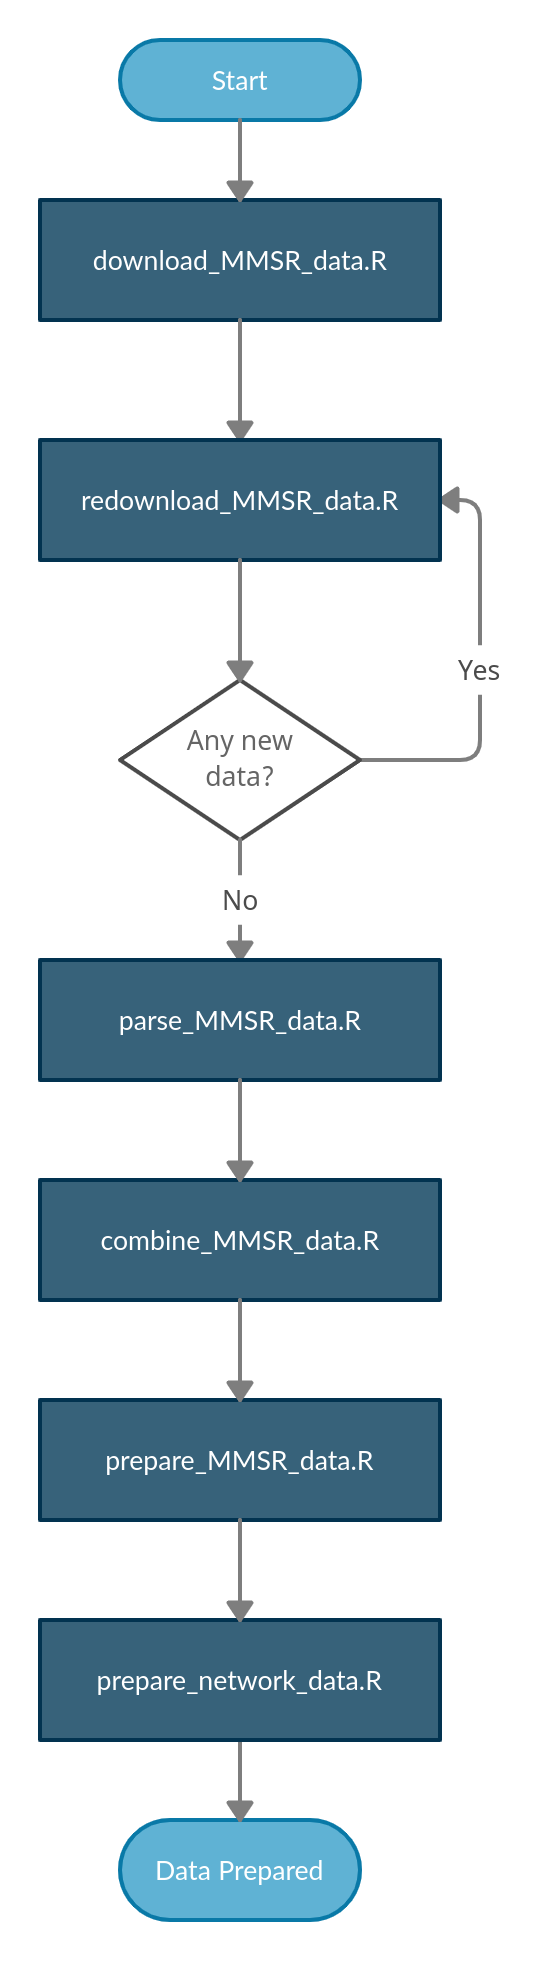
\includegraphics[width=0.75\textwidth]{\detokenize{figures/flowchart_R}}
		\vspace{12pt}
		\caption{The part of the pipeline responsible for downloading, parsing, combining and cleaning the data. Coded in R.}
	\end{subfigure}%
	\begin{subfigure}{.5\textwidth}
		\centering
		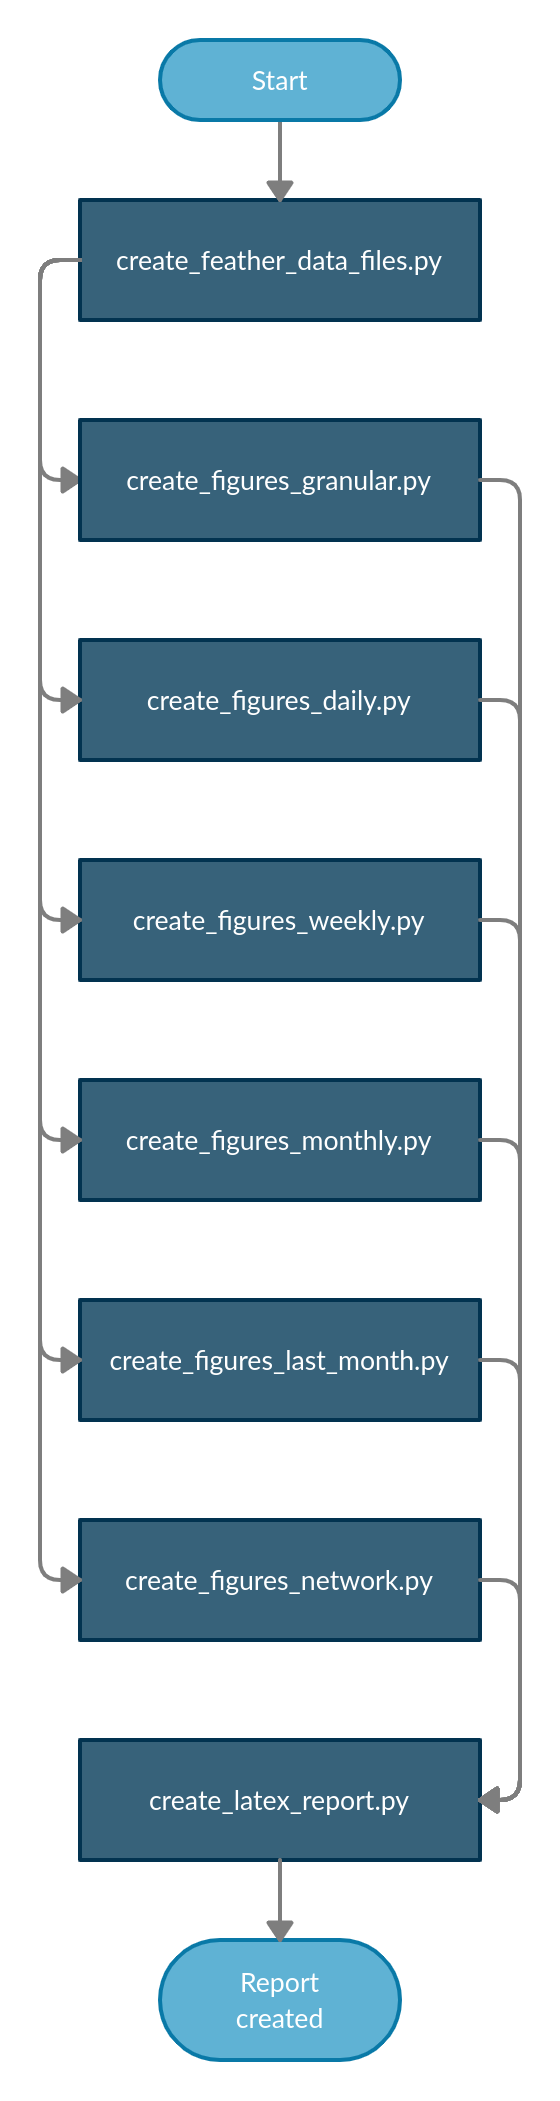
\includegraphics[width=0.735\textwidth]{\detokenize{figures/flowchart_python}}
		\caption{The part of the pipeline responsible for creating lightweight data files, plotting figures and compiling this final pdf report. Coded in Python.}
	\end{subfigure}
	\caption{Graphical visualization of the whole pipeline.}
	\label{fig:technical_summary:flowcharts_R_python}
\end{figure}



\section{Plotting and report compilation}

The figures in this report have been plotted by the python part of the pipeline. The relevant process can be seen on the right hand side of Figure \ref{fig:technical_summary:flowcharts_R_python} while Table \ref{tab:technical_summary:used_functions_python} contains short descriptions of each python function used. I will now describe the process in further detail.


\begin{table}[h]
	\centering
	\begin{tabularx}{0.9\linewidth}{rX}
		Function name & Description \\
		\toprule
		\textbf{create\_feather\_data\_files.py} & Loads the created .csv files, creates new temporal variables, saves different datasets under different granularities. \\
		\textbf{create\_figures\_granular.py} & Creates multiple figures using the full granular dataset.  \\
		\textbf{create\_figures\_daily.py} & Creates multiple figures using the daily dataset.\\
		\textbf{create\_figures\_weekly.py} & Creates multiple figures using the weekly dataset.\\
		\textbf{create\_figures\_monthly.py} & Creates multiple figures using the monthly dataset.\\
		\textbf{create\_figures\_last\_month.py} & Creates multiple figures using the granular dataset containing the last month's transactions.\\
		\textbf{create\_figures\_network.py} & Creates multiple figures using the prepared network centrality dataset.\\
		\textbf{create\_latex\_report.py} & Creates and compiles the final MMSR monthly pdf report.\\
		\textbf{plotting\_functions.py} & Contains definitions and settings of all functions used for figure plotting. \\
		\textbf{config.py} & Contains global variables that are unchanged during the execution of the script such as the root folder path etc.\\
		\bottomrule
	\end{tabularx}
	\caption{Python functions used in the analysis.}
	\label{tab:technical_summary:used_functions_python}
\end{table}

\subsection{Feather data files}
In the first step of this part, we convert the datasets exported with R into a feather file format. The feather file format is a special way of storing data that allows for extremely fast loading / saving. It considerably speeds up our  next computations. For this purpose we use the function \verb|create_feather_data_files.py|. This function:
\begin{itemize}
	\item Loads the relevant granular, daily, weekly and monthly datasets from csv files.
	\item Creates new variables relevant for figure plotting such as year+month, year+quarter etc.
	\item Saves the new files as feather dataframes within a newly created directory structure at:\newline\verb|data/[segment]/data_feather/|.
\end{itemize}

\subsection{Plotting}
In the second step, we use several functions to plot our data. The core of the plotting is coded within the \verb|plotting_functions.py| function and almost in all cases leverages the \verb|seaborn| library. Various different scripts then use these low-level plotting functions to achieve a consistent look of the whole document. These include:
\begin{itemize}
	\item \verb|create_figures_granular.py| - this function leverages the full transaction-level data and produces the associated figures where such transaction-level data is necessary. For instance, all heatmap figures where dependencies between pairs of variables need to be studied are compiled with this function.
	\item \verb|create_figures_daily.py| - this function plots figures where looking at daily quantities is sufficient such as daily volumes, rates and maturities.
	\item \verb|create_figures_weekly.py| - this function plots figures where looking at weekly quantities is sufficient such as daily volumes, rates and maturities.
	\item \verb|create_figures_monthly.py| - this function plots figures where looking at monthly quantities is sufficient such as daily volumes, rates and maturities.
	\item \verb|create_figures_last_month.py| - this function again leverages the full transaction-level data and produces the associated figures where such transaction-level data is necessary. but only for the last month's data. It is used to create figures for chapters summarizing the last month in data.
	\item \verb|create_figures_network.py| - this function plots the figures associated with the network analysis.
\end{itemize}

\subsection{Report compilation}
The third and final step of data visualization entails formatting of this report. I use the \verb|pylatex| python library which allows me to algorithmically generate a latex report and compile via a Python interface. Only the short \verb|report.tex| file within the \verb|/report/| is algorithmically generated, any further chapters and dependencies are fixed and handled with the latex code.


\section{Installation}
Various software and software packages are required to install dependencies for this pipeline. I have strived to make this list of prerequisites as complete as possible but it's very likely there are further steps required that I have forgotten to include.
\begin{itemize}
	\item install RStudio and R
	\item R prompt: install.packages('bizdays')
	\item R prompt: install.packages("readstata13")	
	\item R prompt: install.packages("sqldf")
	\item R prompt: install.packages("XML")
	\item R prompt: install.packages("xml2")	
	\item R prompt: install.packages("httr")
	\item R prompt: install.packages("getPass")
	\item install Anaconda for python
	\item reinstall MikTex
	\item install latexmk package through miktex console
	\item install ActivePerl through the OeppStore
	\item conda prompt: pip install pylatex
	\item conda prompt: pip3 install pandasql
	\item conda prompt: pip3 install pyreadr
	\item conda prompt: pip3 install seaborn==0.11.0
\end{itemize}
